\documentclass[aspectratio = 169, 12pt]{beamer}\usepackage[]{graphicx}\usepackage[]{color}
%% maxwidth is the original width if it is less than linewidth
%% otherwise use linewidth (to make sure the graphics do not exceed the margin)
\makeatletter
\def\maxwidth{ %
  \ifdim\Gin@nat@width>\linewidth
    \linewidth
  \else
    \Gin@nat@width
  \fi
}
\makeatother

\definecolor{fgcolor}{rgb}{0.345, 0.345, 0.345}
\newcommand{\hlnum}[1]{\textcolor[rgb]{0.686,0.059,0.569}{#1}}%
\newcommand{\hlstr}[1]{\textcolor[rgb]{0.192,0.494,0.8}{#1}}%
\newcommand{\hlcom}[1]{\textcolor[rgb]{0.678,0.584,0.686}{\textit{#1}}}%
\newcommand{\hlopt}[1]{\textcolor[rgb]{0,0,0}{#1}}%
\newcommand{\hlstd}[1]{\textcolor[rgb]{0.345,0.345,0.345}{#1}}%
\newcommand{\hlkwa}[1]{\textcolor[rgb]{0.161,0.373,0.58}{\textbf{#1}}}%
\newcommand{\hlkwb}[1]{\textcolor[rgb]{0.69,0.353,0.396}{#1}}%
\newcommand{\hlkwc}[1]{\textcolor[rgb]{0.333,0.667,0.333}{#1}}%
\newcommand{\hlkwd}[1]{\textcolor[rgb]{0.737,0.353,0.396}{\textbf{#1}}}%
\let\hlipl\hlkwb

\usepackage{framed}
\makeatletter
\newenvironment{kframe}{%
 \def\at@end@of@kframe{}%
 \ifinner\ifhmode%
  \def\at@end@of@kframe{\end{minipage}}%
  \begin{minipage}{\columnwidth}%
 \fi\fi%
 \def\FrameCommand##1{\hskip\@totalleftmargin \hskip-\fboxsep
 \colorbox{shadecolor}{##1}\hskip-\fboxsep
     % There is no \\@totalrightmargin, so:
     \hskip-\linewidth \hskip-\@totalleftmargin \hskip\columnwidth}%
 \MakeFramed {\advance\hsize-\width
   \@totalleftmargin\z@ \linewidth\hsize
   \@setminipage}}%
 {\par\unskip\endMakeFramed%
 \at@end@of@kframe}
\makeatother

\definecolor{shadecolor}{rgb}{.97, .97, .97}
\definecolor{messagecolor}{rgb}{0, 0, 0}
\definecolor{warningcolor}{rgb}{1, 0, 1}
\definecolor{errorcolor}{rgb}{1, 0, 0}
\newenvironment{knitrout}{}{} % an empty environment to be redefined in TeX

\usepackage{alltt}
\let\Tiny=\tiny
\usepackage{graphicx}
\usepackage{lmodern}
\usepackage{amsmath, amsthm, amssymb, mathrsfs}
\usepackage{epstopdf}
\graphicspath{{./}{./eps/}}
% these choices affect the slide layout (can be changed)
  \usetheme{Montpellier}
\useoutertheme{infolines}
% modifying the color theme to be scarlet-and-grey for Ohio State (don't change)
\usecolortheme{beaver}
\setbeamercolor{block title}{bg=red!60!black}
\setbeamercolor{block body}{bg=gray!10!white}
\setbeamercolor{item projected}{bg=red!75!black}
\setbeamercolor{subitem projected}{bg=red!90!black}
\setbeamercolor{subsubitem projected}{bg=red!90!black}

% set values for the title slide: [] = text here goes in footer
%                                 {} = text here is on title slide
% logo can have multiple graphics, if necessary
\title[]{Spatial Data and Analysis in R}
\subtitle[]{A PRISM Workshop}
\author[]{Adam Lauretig}
\institute[]{The Ohio State University}
\date{}
\logo{
\includegraphics[height=0.4cm]{OSUlogo.eps}}
\IfFileExists{upquote.sty}{\usepackage{upquote}}{}
\begin{document}

\titlepage     % creates title slide with values defined in header

\section*{Outline}     % starts 'outline' section (TOC, a single slide)

\begin{frame}{Outline}
  \tableofcontents
\end{frame}

\beamerdefaultoverlayspecification{<+->}

\section{Introduction}     % each section (and subsection) title appears on TOC and at top/bottom of slide (theme-dependent)

\begin{frame}{Why Are We Here?}     % frame title appears at top of slide
\begin{itemize}
\item Tobler's first law of geography:
\item ``Everything is related to everything else, but near things are more related than distant things''
\item We want to quantify how the spatial relationship between our observations affect our inferences
\end{itemize}
\end{frame}

\begin{frame}{A Caveat}
\begin{itemize}
\item There are entire disciplines which study these issues (one of them is downstairs)
\item I will be introducing \textit{spatial statistics} with a touch of \textit{GIS}
\item I will not be discussing \textit{GIS} in depth, nor will I discuss remote sensing \textit{at all}
\end{itemize}

\end{frame}


\section{Spatial Data Prep}
\begin{frame}{What are Spatial Data?}
\begin{itemize}
\item Information (attributes) associated with a location
\item Many kinds of spatial data: Points, Lines, Polygons, Raster data
\item Today, we are working with polygon data
\end{itemize}

\end{frame}



\begin{frame}{Prepping our data}
\begin{itemize}
\item Spatial data come in \textit{shapefiles} which are really mini-databases
\item ORDBMS - Linking spatial and attribute data
\item Six parts, all combine to create a map to represent data
\end{itemize}
%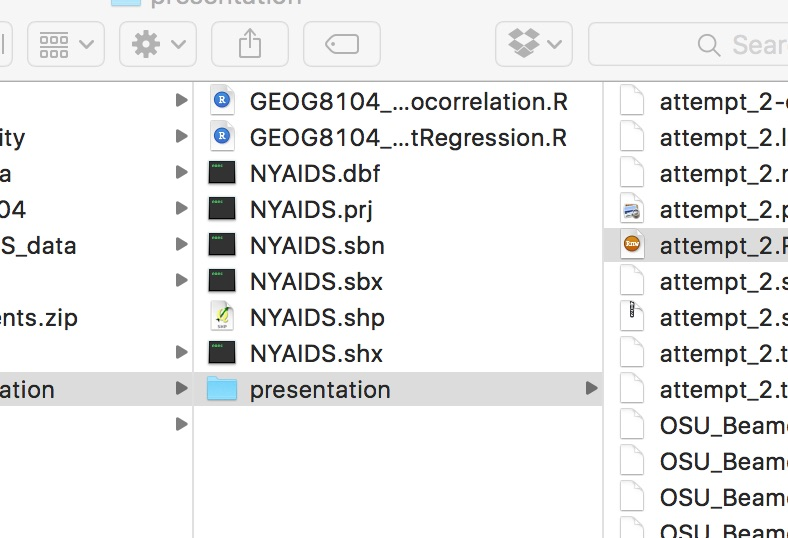
\includegraphics[scale=0.2]{files_screenshot}
\end{frame}

\begin{frame}[fragile]{Loading Our data}
\begin{knitrout}\tiny
\definecolor{shadecolor}{rgb}{0.969, 0.969, 0.969}\color{fgcolor}
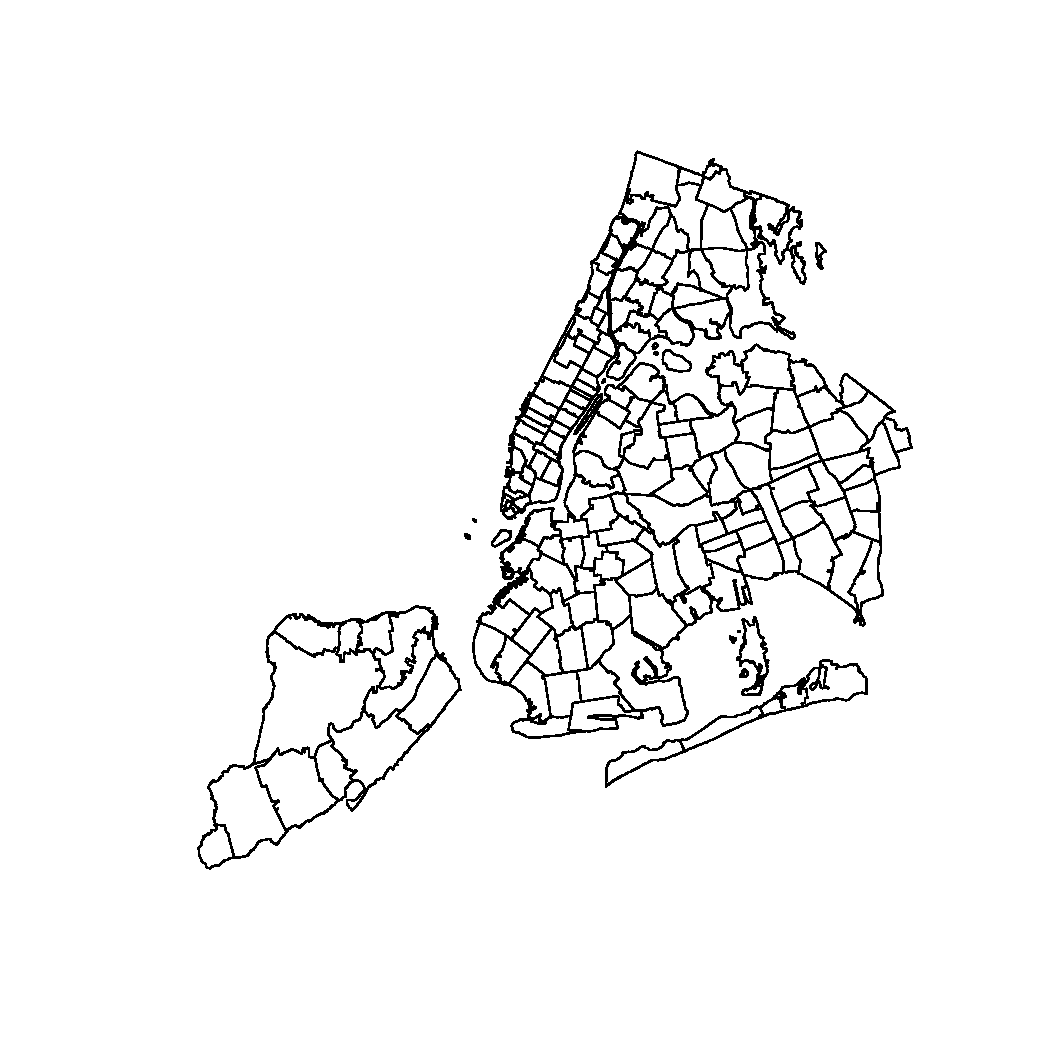
\includegraphics[width=250px]{figure/unnamed-chunk-1-1} 

\end{knitrout}
\end{frame}

\begin{frame}[fragile]{Percent Black}
\begin{knitrout}\tiny
\definecolor{shadecolor}{rgb}{0.969, 0.969, 0.969}\color{fgcolor}
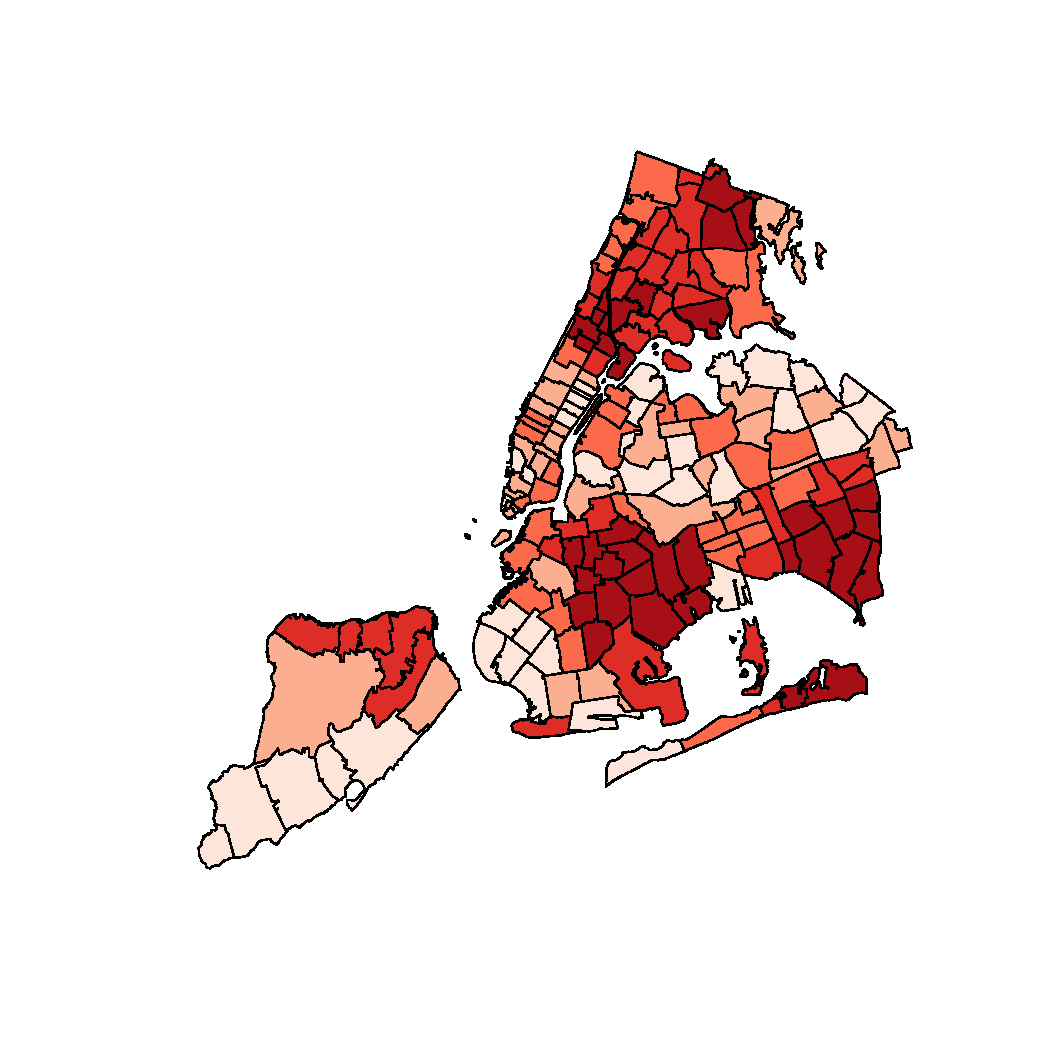
\includegraphics[width=250px]{figure/unnamed-chunk-2-1} 

\end{knitrout}
\end{frame}

\begin{frame}[fragile]{AIDs Rate per 1000 people}
\begin{knitrout}\tiny
\definecolor{shadecolor}{rgb}{0.969, 0.969, 0.969}\color{fgcolor}
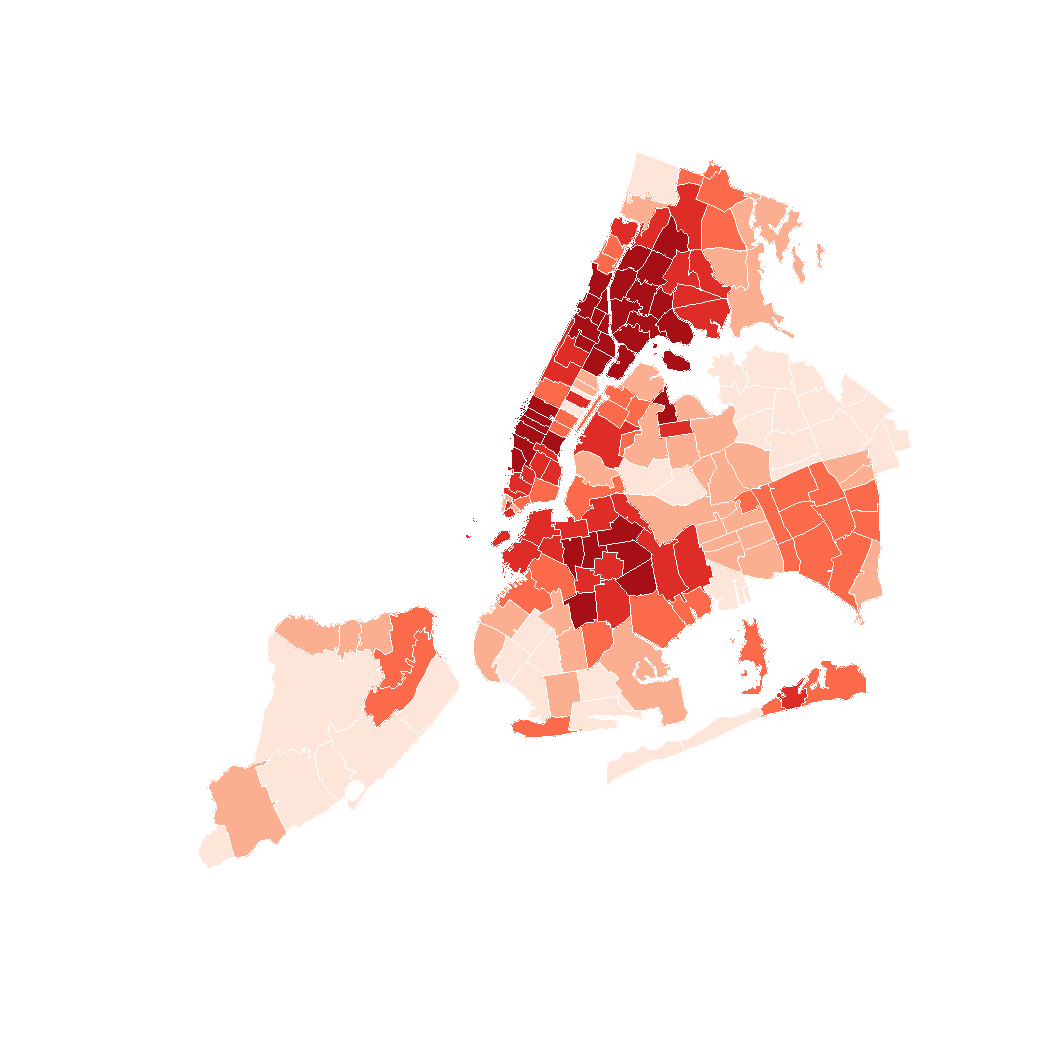
\includegraphics[width=250px]{figure/unnamed-chunk-3-1} 

\end{knitrout}

\end{frame}


\section{Spatial Autocorrelation}
\begin{frame}{Measuring Spatial Autocorrelation}
\begin{itemize}
\item What is spatial autocorrelation?
\item Observations with more similar values tend to occur more closely together
\item Most common test: Moran's I
\end{itemize}
\end{frame}

I's formula is:
\begin{frame}{Formula for Moran's I}
\begin{equation*}
I = \frac{n}{\sum_{i=1}^n \sum_{j=1}^n w_{ij}}
\frac{\displaystyle\sum_{i=1}^n \sum_{j=1}^n w_{ij}(x_i - \bar{x})(x_j -
  \bar{x})}{\displaystyle\sum_{i=1}^n (x_i - \bar{x})^2},\label{eq:morani}
\end{equation*}
where $w_{ij}$ is the weight between observation i and $j$
\end{frame}

\begin{frame}{The Weights Matrix $W$}
\begin{itemize}
\item In Moran's I, there was this thing $w_{ij}$
\item This is the \textit{weights matrix}
\item It allows us to measure the effect neighboring observations $j$ have on our observation of interest i
\item Can be specified in a variety of ways, the simplest of which is binary ("contiguity"): $1$ if observations share a boundary, $0$ if they do not
\item The default in $R$ is ``row standardized,'' where $w_{ij} = \frac{i}{\sum j}$
\end{itemize}
\end{frame}


\begin{frame}[fragile]{Creating a weights matrix in $R$}
\begin{knitrout}\tiny
\definecolor{shadecolor}{rgb}{0.969, 0.969, 0.969}\color{fgcolor}\begin{kframe}
\begin{alltt}
\hlkwd{library}\hlstd{(rgdal)}
\hlkwd{library}\hlstd{(spdep)}
\hlkwd{library}\hlstd{(sp)}
\hlkwd{library}\hlstd{(spatstat)}
\hlstd{file_path} \hlkwb{<-} \hlstr{"/Users/adamlauretig/data/prism_stuff/prism_presentation/NYAIDS_data"}
\hlstd{ny} \hlkwb{<-} \hlkwd{readOGR}\hlstd{(}\hlkwc{dsn} \hlstd{= file_path,}
              \hlkwc{layer} \hlstd{=} \hlstr{"NYAIDS"}\hlstd{,} \hlkwc{verbose}\hlstd{=}\hlnum{FALSE}\hlstd{)}
\hlstd{nygal} \hlkwb{<-} \hlkwd{poly2nb}\hlstd{(ny)} \hlcom{#Create the neighborhood object}
\hlstd{nyQ1.gal} \hlkwb{<-} \hlkwd{nb2listw}\hlstd{(nygal,} \hlkwc{zero.policy}\hlstd{=T)} \hlcom{#Create the weights object}
\end{alltt}
\end{kframe}
\end{knitrout}
\end{frame}

\begin{frame}[fragile]{Running the Moran's I}
% latex table generated in R 3.3.2 by xtable 1.8-2 package
% Wed Mar 22 18:02:10 2017
\begin{table}[ht]
\centering
\begin{tabular}{rrrr}
  \hline
Moran I statistic & Expectation & Variance & p-value \\ 
  \hline
0.68 & -0.01 & 0.00 & 0.00 \\ 
   \hline
\end{tabular}
\label{tab:moranresid}
\end{table}

\end{frame}

\begin{frame}{Where are these clusters?}
\begin{itemize}
\item We can calculate this using a \textit{Local Indicator of Spatial Autocorrelation} (LISA)
\item Measure how similar a value is compared to neighboring values
\item While the Moran's I detects clustering, the LISA detects \textit{clusters}
\end{itemize}
\end{frame}

\begin{frame}[fragile]{Where are these clusters?}
\begin{knitrout}
\definecolor{shadecolor}{rgb}{0.969, 0.969, 0.969}\color{fgcolor}
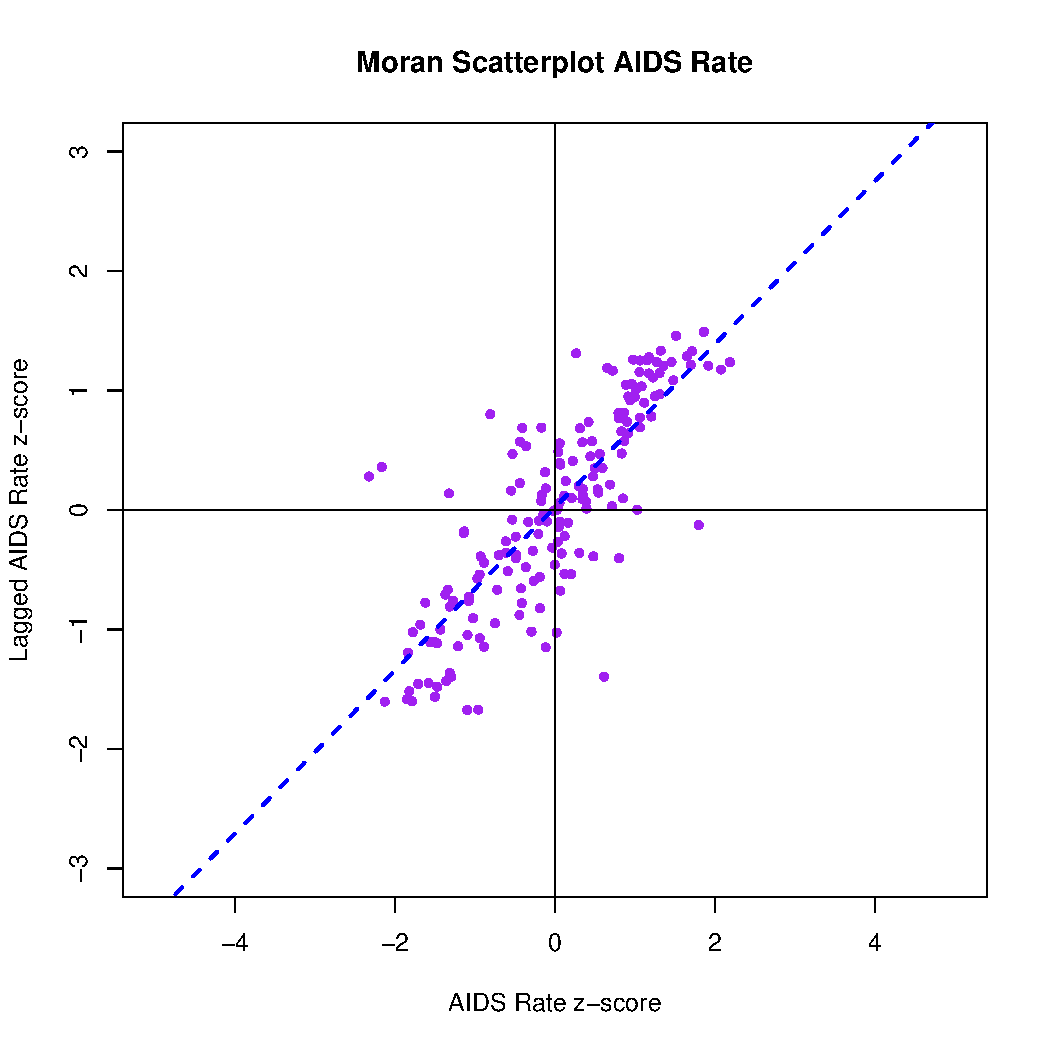
\includegraphics[width=200px]{figure/unnamed-chunk-6-1} 

\end{knitrout}
\end{frame}

\begin{frame}[fragile]{Where are these clusters?}
\begin{knitrout}\tiny
\definecolor{shadecolor}{rgb}{0.969, 0.969, 0.969}\color{fgcolor}
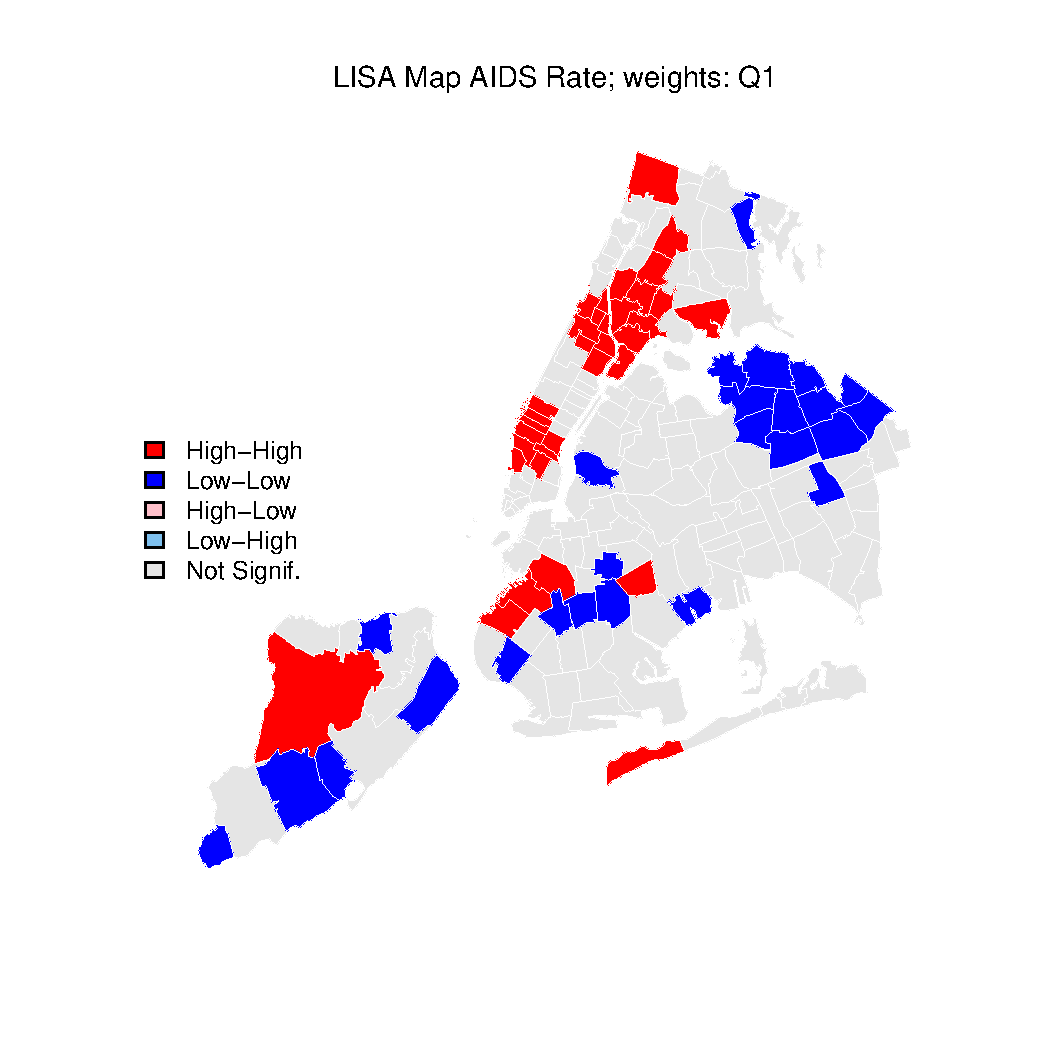
\includegraphics[width=250px]{figure/unnamed-chunk-7-1} 

\end{knitrout}
\end{frame}

\begin{frame}{What About Regression with Spatial Data?}
\begin{itemize}
\item Remember, a key regression assumption is that our observations are IID
\item If there is spatial autocorrelation in our data, we have fewer independent data points than we initially supposed
\item This shrinks our standard errors, making variables appear significant
\item Once we adjust our variance-covariance matrix, previously significant covariates might lose their significance 
\item Addtionally, with spatial autocorrelation, our coefficients may be biased 
\item Two ways of handling this: Spatial Error Models, and Spatial Autoregressive models
\end{itemize}
\end{frame}

\section{Regression}

\begin{frame}{The Math: Spatial Error Model}
\begin{itemize}
\item Normally: $y_i = x_{i}\beta + e_i$, where $e = I(Y- X\beta)$
\item But, we want to model spatial dependence in the residuals
\item $e_{i} = \sum_{j=1}^n w_{ij} + e_{j} + \varepsilon_{i}$, where $w_{ii} = 0$
\item Basically, we regress the error $e_i$ on the surrounding errors
\item We wind up with $e = (I-W)(Y- X\beta)$
\item $\varepsilon$ is the residual of residuals, with $\sum_{\varepsilon} = \sigma^{2}I$
\item The full model: $y_{i} = x_{i}\beta + \sum_{j=1}^{n} w_{ij}e_{j} + \varepsilon_{i}$
\end{itemize}
\end{frame}

\begin{frame}{The Math: Spatial Autoregressive Model}
\begin{itemize}
\item Option 2: the Spatial autoregressive model
\item Instead of lagging the error term, lag $y$, the DV
\item $y_{i} = x_{i}\beta + \sum_{j=1}^{n} w_{ij}y_{j} + \varepsilon_{i}$
\item SAR vs. SEM
\end{itemize}
\end{frame}

\begin{frame}[fragile]{Plain OLS}

\begin{table}
\begin{center}
\scalebox{0.5}{
\begin{tabular}{l c }
\hline
 & Model 1 \\
\hline
(Intercept) & $-3.05^{***}$ \\
            & $(0.80)$      \\
PctWht      & $-0.01^{***}$ \\
            & $(0.00)$      \\
PctHisp     & $0.02^{***}$  \\
            & $(0.00)$      \\
Gini        & $7.97^{***}$  \\
            & $(0.71)$      \\
PctHSEd     & $0.02^{**}$   \\
            & $(0.01)$      \\
PctFemHH    & $0.01$        \\
            & $(0.01)$      \\
\hline
R$^2$       & 0.57          \\
Adj. R$^2$  & 0.55          \\
Num. obs.   & 174           \\
RMSE        & 0.54          \\
\hline
\multicolumn{2}{l}{\scriptsize{$^{***}p<0.001$, $^{**}p<0.01$, $^*p<0.05$}}
\end{tabular}
}
\caption{Statistical models}
\label{table:coefficients}
\end{center}
\end{table}

\end{frame}

\begin{frame}[fragile]{Did we model out our autocorrelation?}
\begin{knitrout}\tiny
\definecolor{shadecolor}{rgb}{0.969, 0.969, 0.969}\color{fgcolor}
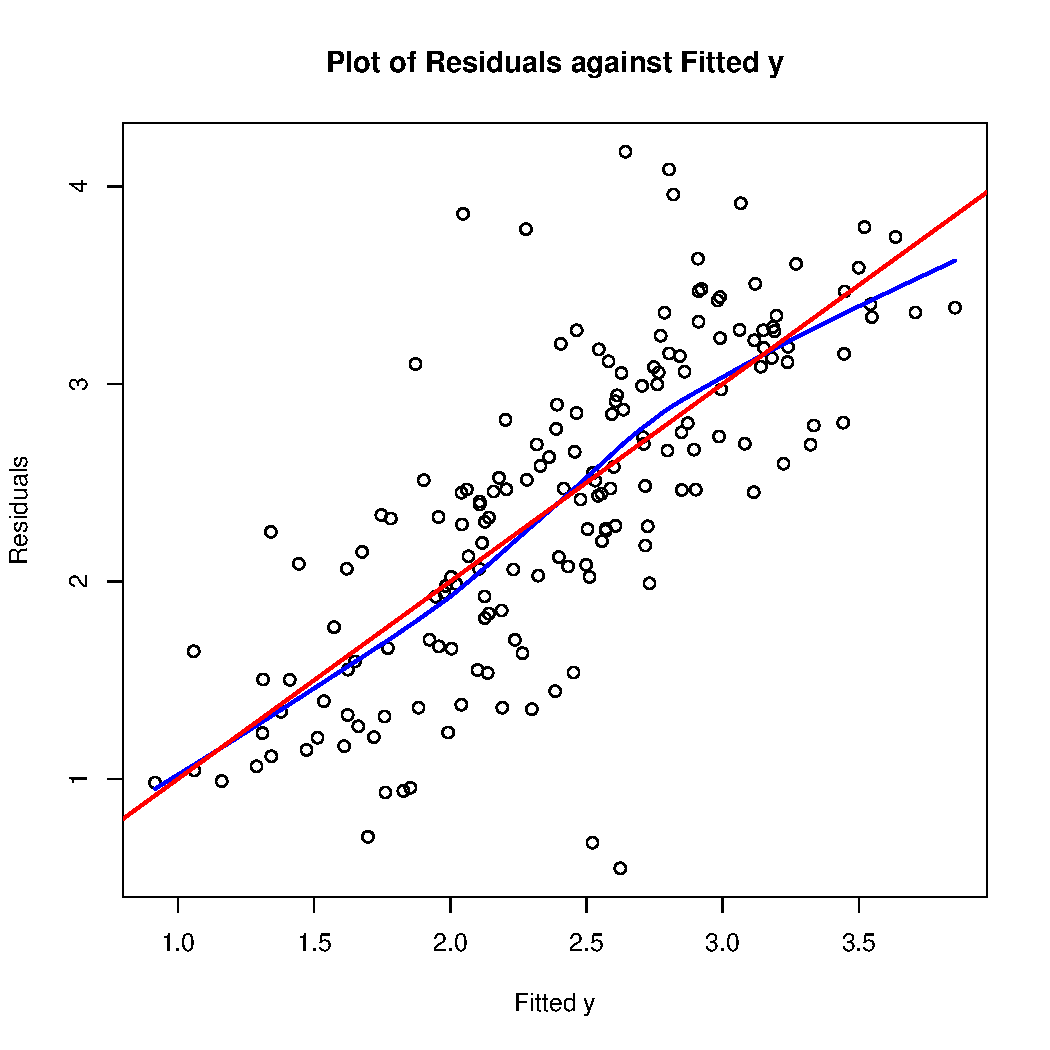
\includegraphics[width=150px]{figure/unnamed-chunk-9-1} 

\end{knitrout}
\end{frame}

\begin{frame}[fragile]{Did we model out our spatial autocorrelation?}
% latex table generated in R 3.3.2 by xtable 1.8-2 package
% Wed Mar 22 18:02:11 2017
\begin{table}[ht]
\centering
\begin{tabular}{rrrr}
  \hline
Moran I statistic & Expectation & Variance & p-value \\ 
  \hline
0.63 & -0.01 & 0.00 & 0.00 \\ 
   \hline
\end{tabular}
\label{tab:moranresid}
\end{table}

No!  This statistic didn't change much from before we ran our regression: $.68$ vs $.63$
\end{frame}

\begin{frame}[fragile]{Where is the residual autocorrelation?}
\begin{knitrout}\tiny
\definecolor{shadecolor}{rgb}{0.969, 0.969, 0.969}\color{fgcolor}
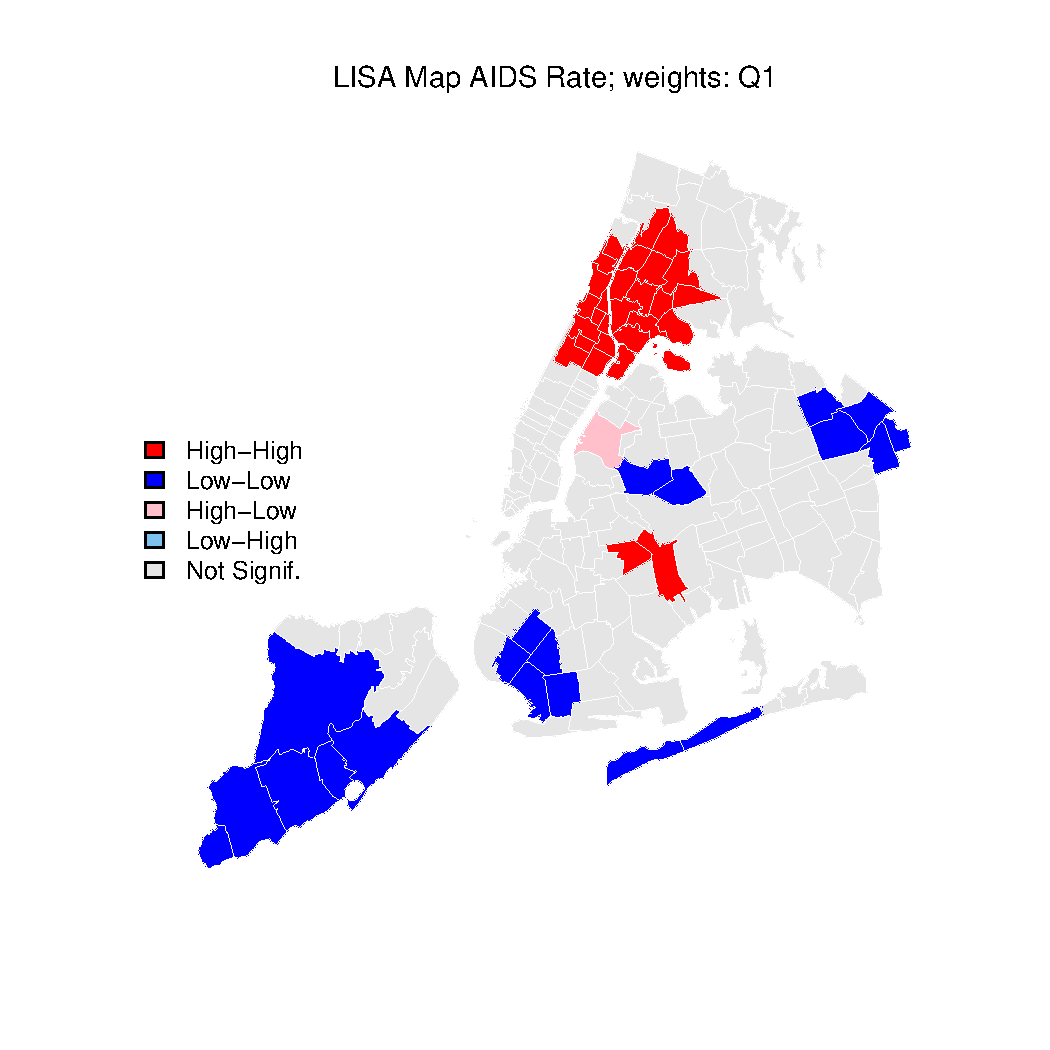
\includegraphics[width=150px]{figure/unnamed-chunk-11-1} 

\end{knitrout}
\end{frame}

\section{Spatial Regression}
% \begin{frame}[fragile]{Picking a model}
% <<echo = FALSE, out.width='150px', dpi=500, size = "tiny", cache = TRUE, message=FALSE, warning=FALSE>>=
% suppressMessages(library(rgdal))
% suppressMessages(library(spdep))
% suppressMessages(library(sp))
% suppressMessages(library(spatstat))
% file_path <- "/Users/adamlauretig/data/prism_stuff/prism_presentation/NYAIDS_data"
% ny <- readOGR(dsn = file_path, 
%               layer = "NYAIDS", verbose=FALSE)
% ny <- ny[-c(38),]
% nygal <- poly2nb(ny) #Create the neighborhood object
% nyQ1.gal <- nb2listw(nygal, zero.policy=T)
% lrate <- log1p(ny$Rate1000)
% reg1 <- lm(lrate ~ PctWht + PctHisp + Gini + PctHSEd + PctFemHH, data = ny)
% 
% # Lagrange multiplier test for model fit
% lmtest_out <- lm.LMtests(reg1, nyQ1.gal, test=c("LMerr", "LMlag"))
% texreg::texreg(l = list(lm.LMtests(reg1, nyQ1.gal, test=c("LMerr", "LMlag"))))
% 
% @
% \end{frame}
\begin{frame}{Can we Model this Spatial Autocorrelation}
\begin{itemize}
\item One option is to use fixed effects
\item But this removes something interesting -- the spatial relationship
\item Another option is to explicitly model the spatial relationship
\end{itemize}
\end{frame}
\begin{frame}[fragile]{Spatial Autoregressive Model}

\begin{table}
\begin{center}
\scalebox{0.5}{
\begin{tabular}{l c }
\hline
 & Model 1 \\
\hline
(Intercept)         & $-1.52^{*}$   \\
                    & $(0.63)$      \\
PctWht              & $-0.01^{***}$ \\
                    & $(0.00)$      \\
PctHisp             & $0.01^{**}$   \\
                    & $(0.00)$      \\
Gini                & $4.48^{***}$  \\
                    & $(0.64)$      \\
PctHSEd             & $0.01$        \\
                    & $(0.01)$      \\
PctFemHH            & $0.00$        \\
                    & $(0.01)$      \\
$\rho$              & $0.54^{***}$  \\
                    & $(0.06)$      \\
\hline
Num. obs.           & 174           \\
Parameters          & 8             \\
Log Likelihood      & -101.93       \\
AIC (Linear model)  & 285.72        \\
AIC (Spatial model) & 219.85        \\
LR test: statistic  & 67.86         \\
LR test: p-value    & 0.00          \\
\hline
\multicolumn{2}{l}{\scriptsize{$^{***}p<0.001$, $^{**}p<0.01$, $^*p<0.05$}}
\end{tabular}
}
\caption{Statistical models}
\label{table:coefficients}
\end{center}
\end{table}

\end{frame}

\begin{frame}[fragile]{Spatial Error Model}

\begin{table}
\begin{center}
\scalebox{0.5}{
\begin{tabular}{l c }
\hline
 & Model 1 \\
\hline
(Intercept)         & $-0.28$      \\
                    & $(0.88)$     \\
PctWht              & $-0.01^{**}$ \\
                    & $(0.00)$     \\
PctHisp             & $0.01^{**}$  \\
                    & $(0.00)$     \\
Gini                & $4.25^{***}$ \\
                    & $(0.90)$     \\
PctHSEd             & $0.01$       \\
                    & $(0.01)$     \\
PctFemHH            & $0.01$       \\
                    & $(0.01)$     \\
$\lambda$           & $0.66^{***}$ \\
                    & $(0.06)$     \\
\hline
Num. obs.           & 174          \\
Parameters          & 8            \\
Log Likelihood      & -107.85      \\
AIC (Linear model)  & 285.72       \\
AIC (Spatial model) & 231.70       \\
LR test: statistic  & 56.01        \\
LR test: p-value    & 0.00         \\
\hline
\multicolumn{2}{l}{\scriptsize{$^{***}p<0.001$, $^{**}p<0.01$, $^*p<0.05$}}
\end{tabular}
}
\caption{Statistical models}
\label{table:coefficients}
\end{center}
\end{table}

\end{frame}

\begin{frame}[fragile]{Comparing Findings - OLS}
\begin{knitrout}\tiny
\definecolor{shadecolor}{rgb}{0.969, 0.969, 0.969}\color{fgcolor}
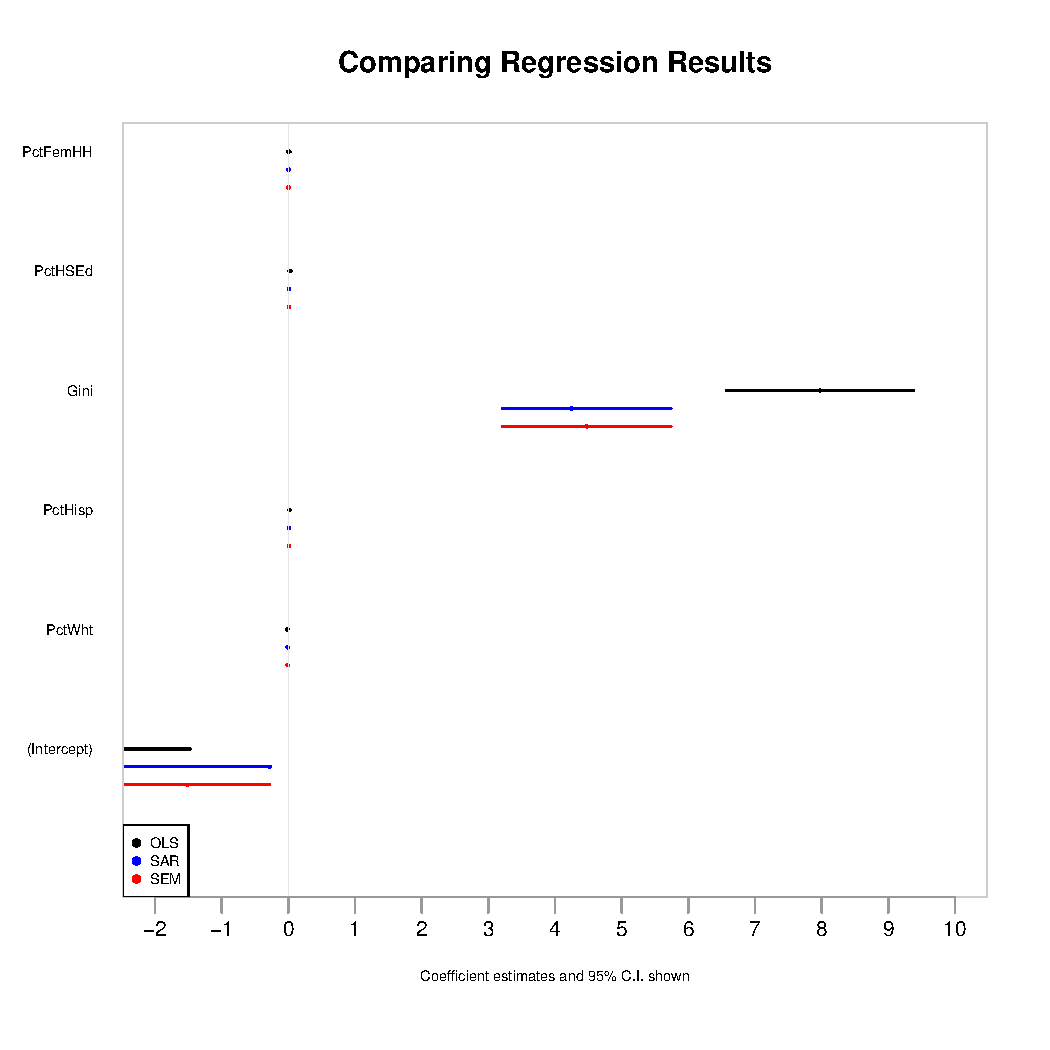
\includegraphics[width=200px]{figure/unnamed-chunk-14-1} 

\end{knitrout}
\end{frame}

\begin{frame}[fragile]{Did These Resolve our Spatial Autocorrelation?}
% latex table generated in R 3.3.2 by xtable 1.8-2 package
% Wed Mar 22 18:14:10 2017
\begin{table}[ht]
\centering
\begin{tabular}{rrrr}
  \hline
Moran I statistic & Expectation & Variance & p-value \\ 
  \hline
-0.10 & -0.01 & 0.00 & 0.08 \\ 
   \hline
\end{tabular}
\label{tab:moranresid2}
\end{table}

YES!
\end{frame}

\begin{frame}{Conditional Autoregressive Model (CAR)}
\begin{itemize}
\item Model the spatial relationship according to a Markov Random Field (MRF)
\item Each observation depends only on values at neighboring locations, not glocal values
\item Written out:
\item $c_{ij}$ is the weight matrix
\item $$ E(y_i | y_{-i}) = x_i \beta + \sum_{j=1}^n + c_{ij} [ y_j - x_i \beta ] $$
\item $$ \text{var}(y_i | y_{-i}) = \sigma_{i}^2 $$
\end{itemize}
\end{frame}


\begin{frame}{Conditional Autoregressive Model (CAR) (cont'd)}
\begin{itemize}
\item This defines a joint multivariate normal distribution with variance
\item $$ \sum_Y = (I - C)^{-1} \sum_{C} $$
\item $$ \sum_{CAR} = \sigma^{2} (I - C)^{-1} V_{C} $$
\item $$ = \sigma^{2}V_{CAR} $$
\end{itemize}
\end{frame}


\begin{frame}{SAR vs. CAR}
\begin{itemize}
\item SAR: $$ y_i \sim N(0, (I-W)^{-1} D^{\sim} (I-W)'^{-1}) $$
 $$ \sigma_{SAR} = \sigma^{2} (I - W)^{-1} V_{\epsilon} (I - W')^{-1} $$
\item CAR: $$ y_i \sim N(0, (I-C)^{-1} D )$$
 $$ \sum_{CAR} = \sigma^{2} (I - C)^{-1} V_{C} $$
\end{itemize}
\end{frame}



\begin{frame}{Workflow for Spatial Regression}
\begin{itemize}
\item In addition to normal EDA, do some ESDA (Exploratory Spatial Data Analysis), mapping out variables
\item Check for spatial autocorrelation
\item Run your normal regression, with the variables you think are necessary
\item Check once more for spatial autocorrelation, in your residuals
\item If there's still autocorrelation, run a spatial model
\item One final check for autocorrelation in your residuals
\end{itemize}
\end{frame}

\section{Discussion}
\begin{frame}{Where Can we Apply These Methods in Political Science}
\begin{itemize}
\item Voting and Political Behavior patterns (Data available at the Census Tract level (or less))
\item Agricultural/industrial data (economic output)
\item Conflict/Political Violence data (ex: ACLED)
\item Anything with an address or lon/lat coordinates can be georeferenced
\item
\end{itemize}
\end{frame}

\begin{frame}{Other tools}
\begin{itemize}
\item CAR Models
\item Spatial/Spatio-temporal scan statistics
\item Geographically Weighted Regression
\item Kernel Density Estimation
\item Kriging/Geostatistics
\item Spatio-temporal approaches
\end{itemize}
\end{frame}

\begin{frame}{Resources}
\begin{itemize}
\item Yuri Zhukov's Spatial Workshop: \url{http://www.people.fas.harvard.edu/~zhukov/spatial.html}
\item Brunsdon, Chris, and Lex Comber. \textit{An introduction to R for spatial analysis \& mapping.} Sage, 2015.
\item Bivand, Roger S., and Edzer J. Pebesma. \textit{Applied Spatial Data Analysis with R.} Springer, 2013.
\item Waller, Lance A., and Carol A. Gotway. \textit{Applied spatial statistics for public health data.} John Wiley \& Sons, 2004.
\item Cressie, Noel. \textit{Statistics for spatial data.} John Wiley \& Sons, 1993.
\end{itemize}
\end{frame}

\begin{frame}{Acknowledgements}
Thank you to Will Massengill and Drew Rosenberg for this opportunity, and to Elisabeth Root, whose code I drew heavily from
\end{frame}


\section*{References}     % use '*' on section/subsection to keep it off TOC

\begin{frame}{References}

\end{frame}

\section*{Appendix}     % extra slides in appendix, but these sections/subsections shouldn't be in TOC (use '*')
\subsection*{}

\begin{frame}{}
\end{frame}

\end{document}
